\section{Berechnung der Dense Units}
\label{sec:chap3}

Cluster von benachbarten Punkten müssen zu minPoint großen Subsets kombiniert werden. Diese Subsets werden Dense Units genannt.
Dense Units werden in verschiedene Funktionen mit unterschiedlichen Zwecken berechnet. Das Hauptziel dieser Berechnung ist die Bestimmung einer Teilmenge aus allen möglichen Kombinationen in einem Subset. Dabei dürfen keine Wiederholungen der Dense Units auftreten. Die Anzahl an Kombinationen aus einem Subset können mittels dem Binominialkoeffizient $\binom{n}{k}$ berechnet werden. Dabei ist \emph{n} die Anzahl der Elemente in dem Subset und \emph{k} die minimale Anzahl an Punkten in einem Subset (e.g. minPoints). Daraus entstehen k-Elemente großes Subsets von einem n-Elemente Set ohne Wiederholungen der Kombinationen.
Wenn ein Core Set aus folgenden Punkten besteht: [1, 5, 7, 9, 22] und die minimale Anzahl an Punkten in einem Subset Drei ist, sind die ersten drei Dense Units folgende: [1, 5, 7] und [1, 5, 9] und [1, 5, 22]. Die Formel zur Berechnung der Dense Units kann also folgendermaßen betrachtet werden: 
$ \binom{|CS|}{minPoints}$ \cite{7022654} Abbildung \ref{dense-calculation} zeigt ein weiteres Beispiel für n-Punkte in einem Core Set mit minPoints von 4.

\begin{figure}
	\centering
	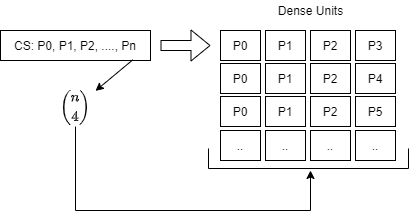
\includegraphics[width=0.5\textwidth]{DenseUnitBerechnung.png}
	\caption{Berechnung der Dense Units}
	\label{dense-calculation}
\end{figure}